\section{Résultats & discussion}
\subsection{Analyse de la variabilité expérimental et levée d'ambiguité sur l'alignement}
 
Il est intéressant de vérifier  si les deux outils d’alignement diffèrent significativement dans  
leur capacité à aligner de manière unique les lectures. Dans un premier temps j'ai construit à partir de mon fichier tabulé issue du script Bash  Pour ce faire, j’ai réalisé une analyse statistique sur les proportions relatives des lectures uniques par patient.  
J’ai commencé par effectuer un test de normalité de Shapiro-Wilk~\textsuperscript{\cite{shapiro_wilk_1965}} sur les données de proportions de lectures uniques pour chaque outil,  
afin de vérifier l’hypothèse de normalité nécessaire à l’utilisation d’un test paramétrique.~\textsuperscript{\cite{statistical_test_2021}}

Les résultats du test ne m’ont permis de rejeté cette hypothèse ; j’ai donc opté pour une approche non paramétrique plus robuste : le test de Wilcoxon ~\textsuperscript{\cite{wilcoxon_signed_rank_1945}} pour échantillons appariés.  

Il permet de comparer les distributions des proportions de lectures uniques entre \texttt{STAR} et \texttt{CRAC}, tout en tenant compte de la structure appariée des données (chaque patient servant de contrôle pour lui-même en quelque sorte).

Mon objectif est ici de déterminer si les différences observées dans les taux d’alignement unique relèvent de fluctuations aléatoires ou d’une divergence systématique entre les deux méthodes d’alignement. Pour autant il ne s'agit pas d'une comparaison d'outil en bon et due forme, mais de regarder grossièrement dans qu'elle mesure deux stratégies différentes pourraient influer sur la profondeur de lectures alignés. Subsidiairement, si il existe une significativité, est ce que cela peut influer en tout ou partie sur la variabilité des unités de comptages (nombres de lectures alignés à une position). 

\begin{figure}[H]
\begin{flushleft}
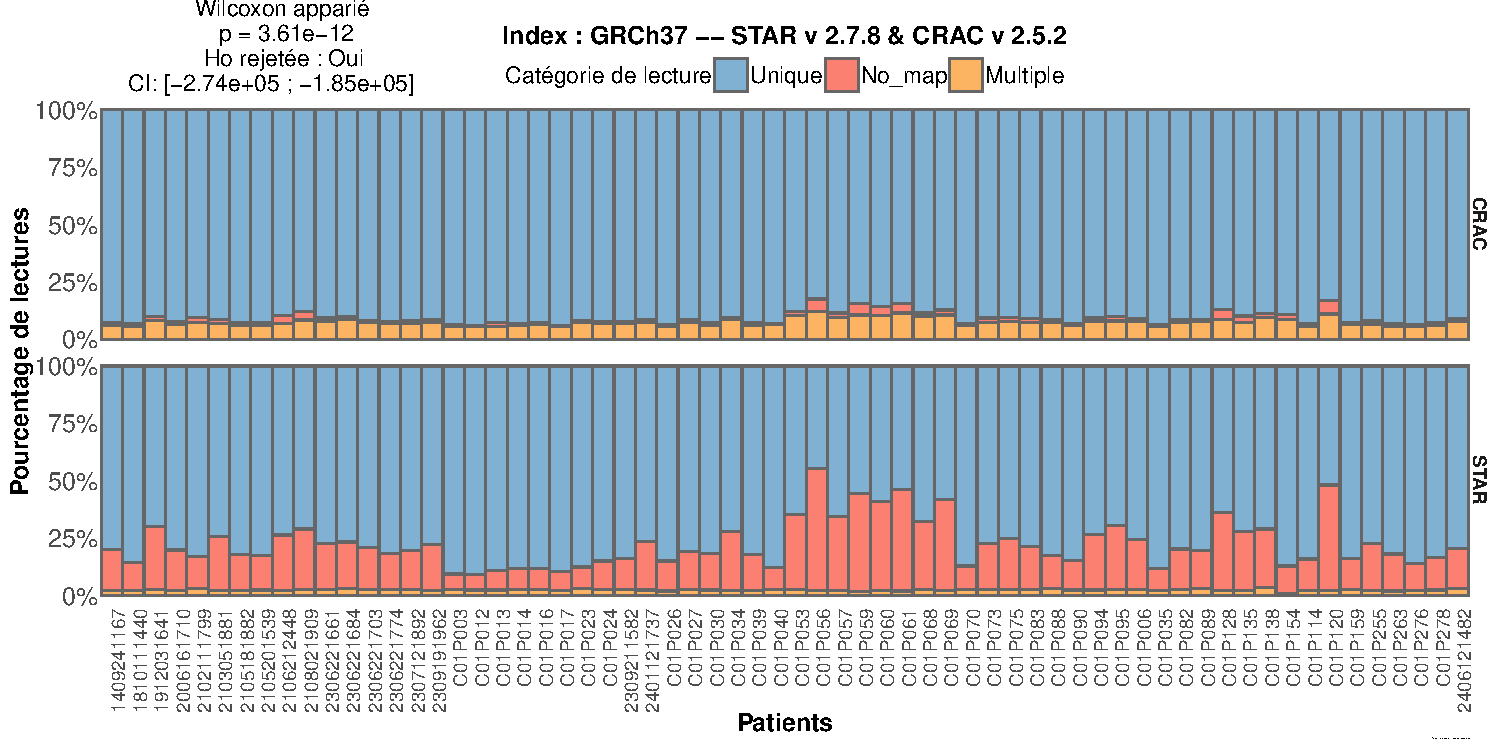
\includegraphics[width=1\linewidth]{Figure_STAR_CRAC_P.pdf}
\caption{\underline{Comparaison des profils d'alignement par patient entre STAR et CRAC}}
\label{fig:mappingp}
\end{flushleft}
\end{figure}

Soulignons ces résultats ne reflètent pas nécessairement une différence de qualité dans l’alignement entre \texttt{STAR} et \texttt{CRAC}. Comme évoqué précédemment, les stratégies algorithmiques diffèrent, notamment dans la manière de classifier les lectures uniques, multiples, et enfin celles non mappées. Ces divergences peuvent influencer la sensibilité de détection à certains types de variants.

\begin{figure}[H]
\begin{center}
\resizebox{1.05\textwidth}{!}{  
    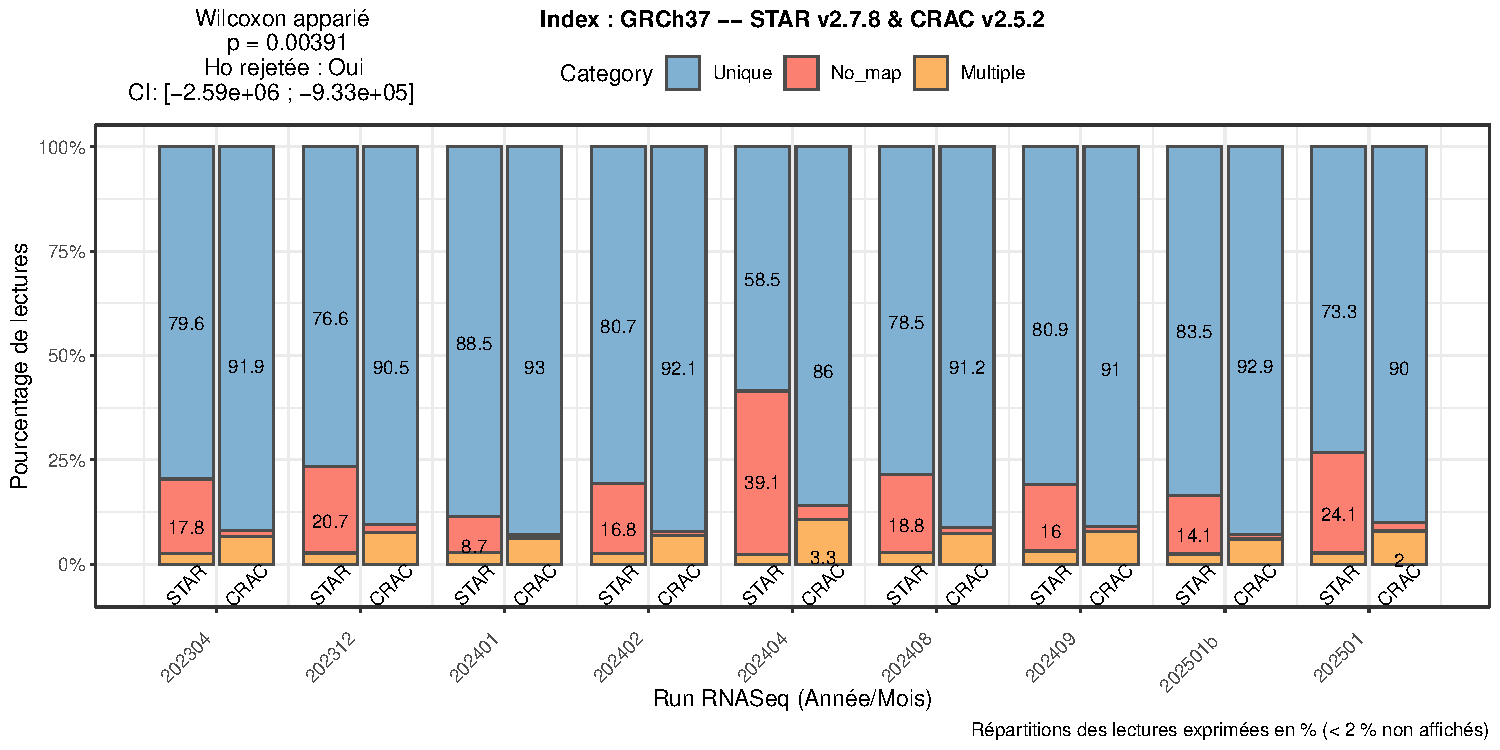
\includegraphics[width=1\linewidth]{Figure_STAR_CRAC_R.pdf}}
    \caption{\underline{Profils d'alignements par run entre STAR et CRAC}}
    \label{fig:mappingr}
\end{center}
\end{figure}

L'analyse statistique par test de Wilcoxon apparié révèle une différence significative entre le nombre de lectures uniques alignées par STAR et CRAC (\( p = 0{,}00391 \)). L'intervalle de confiance négatif \([-2{,}59 \times 10^{6} ; -9{,}33 \times 10^{5}]\) nous indique que \texttt{CRAC} (dans le paramétrage par défaut et pour notre cas d'étude précis) génère de manière systématique un nombre de lectures alignées de manière unique significativement plus élevé que \texttt{STAR} pour un même échantillon. Ce résultat suggère soit une sensibilité accrue, soit une stratégie d’alignement plus permissive. Par conséquent, même si la proportion de lectures uniques est  globalement comparable entre les deux outils (conclusion que l'on peut admettre autant à l'échelle du patient (\textbf{figure \ref{fig:mappingp}}) qu'a l'échelle du \textit{run} RNASeq \textbf{figure \ref{fig:mappingr}}. Avant d'éffectuer des analyses de quantification, j’ai mené des explorations complémentaires en extrayant la métrique nommée \og NH \fg (\textit{Number of Hits}), cette information est un champ dans le fichier de sortie au format \texttt{SAM}. Pour ce faire, j’ai développé un script Bash (cf. \textbf{Annexe à ajouter}). L'intérêt ici est d'essayer de comprendre la différence de lectures uniques entre les deux outils. 



    Statistiques descriptives sur la profondeur de lecture, par run et par échantillon.
    Mise en évidence de la non-reproductibilité : inter-run vs. intra-run.
    Visualisations pour illustrer la disparité de couverture.

    Présentation de STAR et CRAC :
    Méthodologie, hypothèses sous-jacentes, différences de traitement.

    Alignement des mêmes échantillons avec les deux outils.

    Comparaison des métriques de mapping : taux d’alignement unique/multiple/non-aligné.

    Conclusion : validation que l’étape d’alignement n’est pas responsable de la variabilité observée.


\subsection{Analyse des données de comptages avec normalisation TPM}



\subsection{Analyse des données de comptages avec normalisation TMM}

    Le test évalue si, pour un gène donné, l’expression normalisée (CPM\_TMM) est stitistiquement différente entre les conditions (ex: patients vs contrôles).
    Une p-value faible (<0.05 généralement) indique que la différence observée est peu probable due au hasard, donc potentiellement biologiquement significative.
    Ce test est robuste face aux distributions non normales, ce qui est fréquent en RNA-seq.
    Cependant, ce test ne donne pas d’indication sur la taille de l’effet (seulement s’il y a une différence significative).
    Sur 56 tests (un par gène), il faut ajuster la p-value pour réduire les faux positifs.
    
Modalités de calcul du test Wilcoxon (Mann-Whitney)
    Classe toutes les valeurs des deux groupes combinés (conditions) par ordre croissant.
    Attribue un rang à chaque valeur.
    Calcule la somme des rangs pour un groupe.
    Compare cette somme avec la distribution attendue si les deux groupes venaient de la même population.
    La p-value correspond à la probabilité d’obtenir une somme de rangs aussi extrême (ou plus) sous l’hypothèse nulle (pas de différence entre conditions).
Graphique
 j'affiche la distribution des CPM normalisés par gène, par condition, avec des points colorés.
    L’annotation avec label permet d’afficher la p-value pour chaque gène, informant visuellement sur la significativité des différences observées.
    Cela m’aide à relier visuellement l’intensité d’expression avec la signification statistique.
    
L’absence de différences statistiquement significatives (p > 0.05) dans les niveaux d’expression normalisés (CPM TMM) des 56 gènes d’intérêt entre les conditions étudiées suggère que, au sein des échantillons analysés, ces gènes ne présentent pas de variations d’expression marquées ou robustes en lien avec le facteur expérimental considéré. Cela peut indiquer que, dans ce contexte biologique précis, la modulation transcriptionnelle de ces gènes n’est pas significativement impactée par la condition testée, ou que les effets sont trop faibles pour être détectés avec la taille d’échantillon actuelle. Il est aussi possible que la variabilité inter-individuelle ou technique masque de potentielles différences subtiles. Enfin, ces résultats invitent à considérer d’autres niveaux de régulation (post-transcriptionnel, épigénétique) ou des approches complémentaires (ex. analyses multi-omics, échantillonnages plus larges) pour mieux comprendre les mécanismes biologiques sous-jacents dans cette pathologie ciblée.

   
    

